%%%%%%%%%%%%%%%%%%%%%%%%%%%%%%%%%%%%%%%%%%%%%%%%%%%%%
%				 Coprocessor module					%
%					-----------						%
% Author: Theodoros Theodoropoulos&Adrian Schindler %
%%%%%%%%%%%%%%%%%%%%%%%%%%%%%%%%%%%%%%%%%%%%%%%%%%%%%


\section{Coprocessor}


The following section describes the inner structure of the coprocessor.

It comprises a subsection regarding the incremental calculation module, and subsections regarding the buffer management and the interpolation.

\begin{figure}[h]
\center
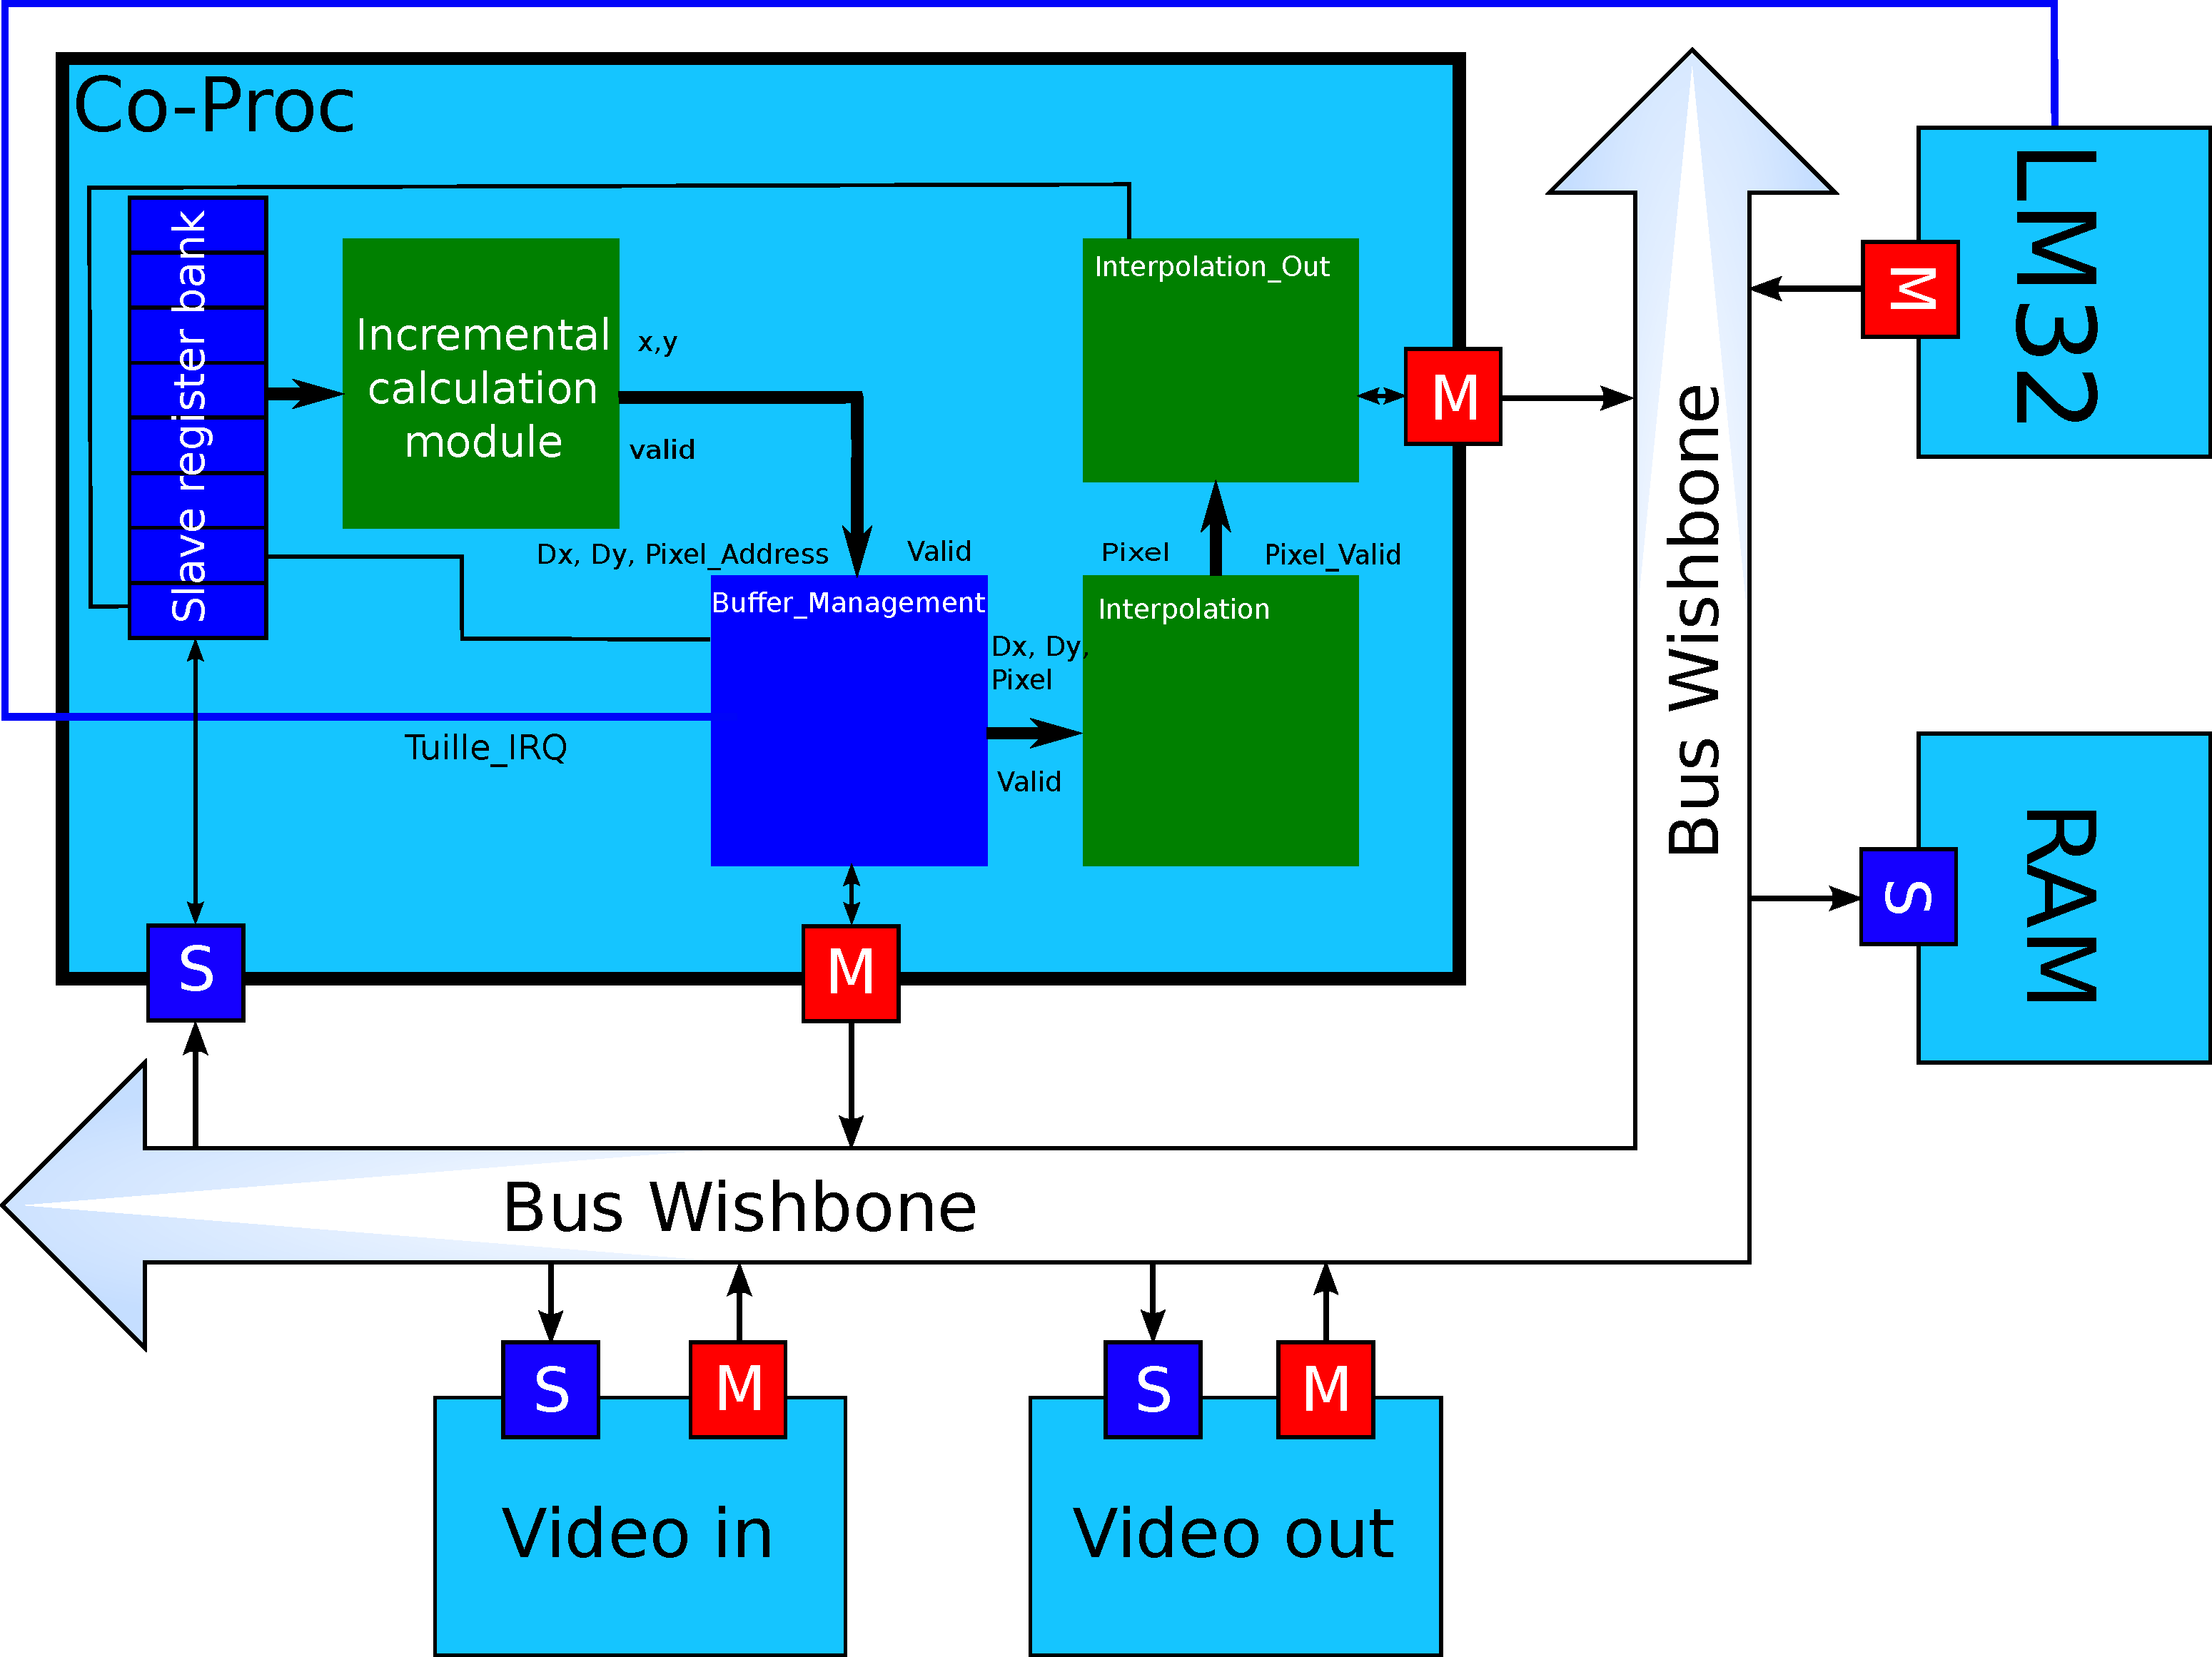
\includegraphics[width=11cm]{figs/copro2.pdf}
\caption{Coprocessor's inner structure}
\label{coproc_struct}
\end{figure}

\subsection{Calculation module}

\subsubsection{Incremental module}

\begin{figure}[H]
\center
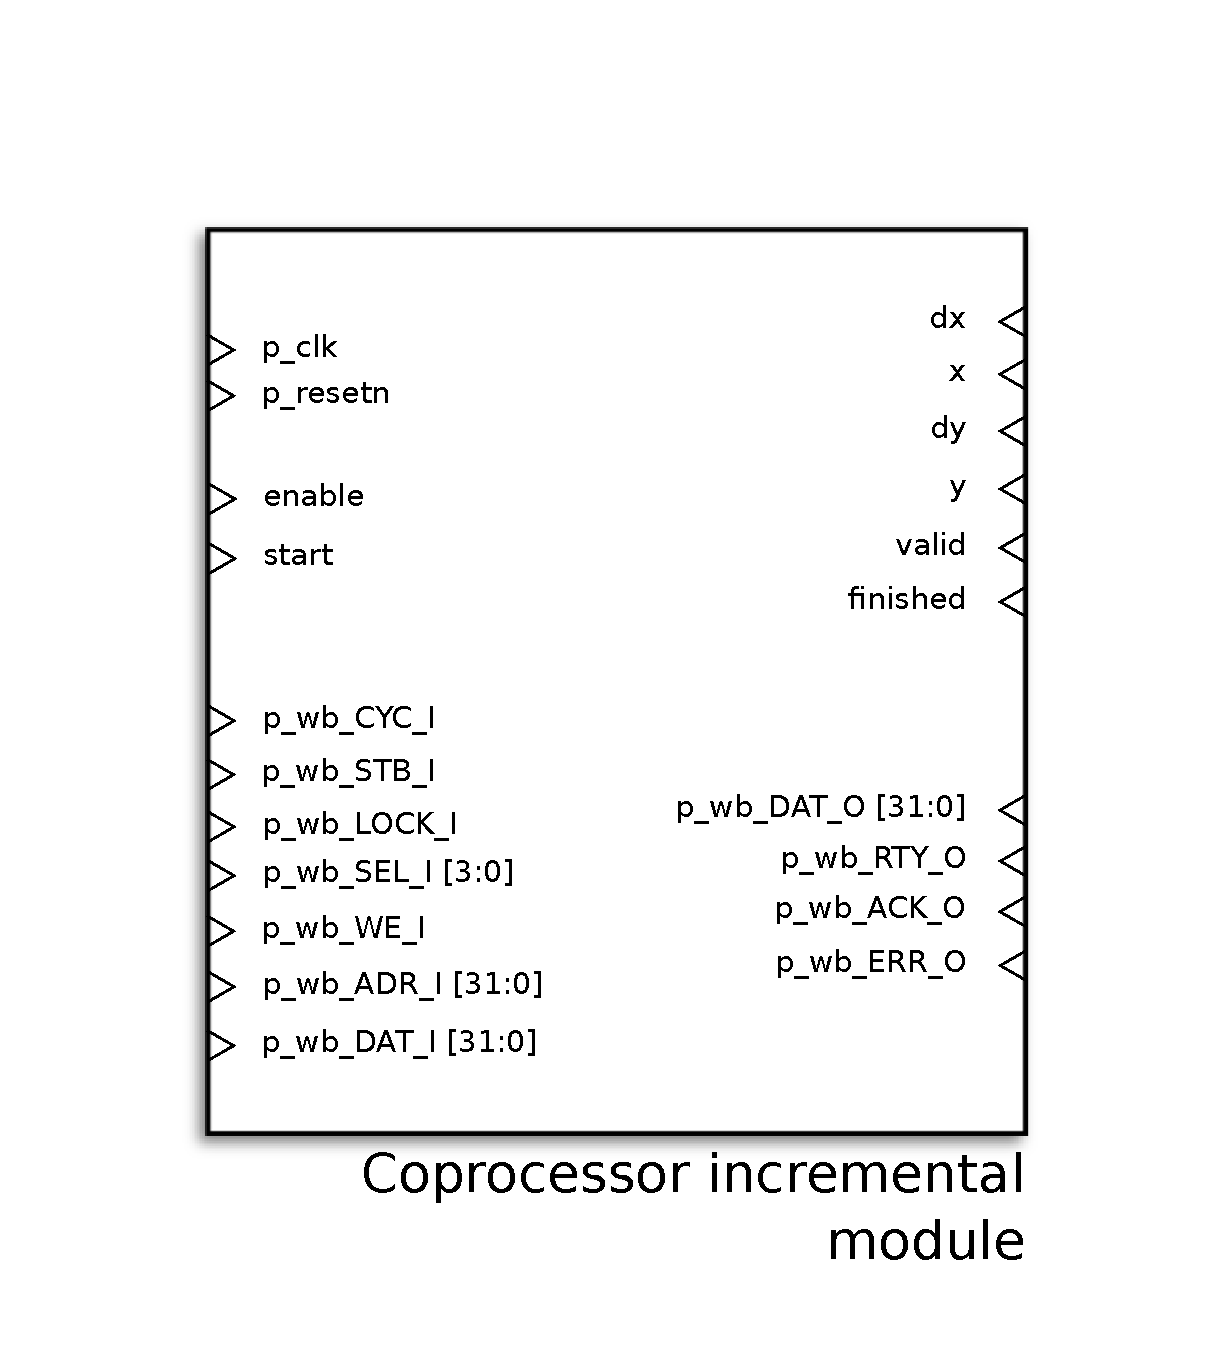
\includegraphics[width=7cm]{figs/coproc_incr_symbol.pdf}
\caption{Coprocessor incremental calculation module's input/output ports}
\label{Incr_interface}
\end{figure}


The incremental calculation module consists of one clock-triggered process. Unlike other modules which work on an entire image it works on a tile-by-tile basis: It loads the coefficients for the new tile and then outputs the 16 x 16 pixels. Data is stored in the mfixed format, however, the version provided on the SEN website (\url{http://sen.enst.fr/ue/elec342/v_fixe}) has been modified to be C++ compatible and work with SystemC. We transformed the C union into a class with two private values which can be extracted by two public functions; in line with object-oriented programming concepts. For ease of use, we also added the $+$ and $=$ operator which internally use fx\_add and fx\_copy. In addition, we added functions for debug purposes: the \texttt{<}\texttt{<} operator for command line output and sc\_trace for signal tracing.

The functionality of the module can be enabled/disabled via the \texttt{enable} signal. This does also work in the middle of a calculation, for instance during the calculation process of a tile. There are three states which are traversed during the calculation of any tile illustrated in figure \ref{incr_sm} and enumerated as follows:

\begin{itemize}
\item State 0: If the start signal is high, the coefficients are loaded from the wishbone slave interface (which have been written there by the LM32 beforehand) to an internal register for each coefficient. We had to typecast the uint32\_t value output by the wishbone interface to mfixed which does not cause any problem since the upper portion of the mfixed type (which represents the digit) is unsigned. Once the start signal passes to low, the calculation will begin and the module passes to state 1.
\item State 1: In this state, the coprocessor outputs one pixel per clock cycle. It indicates this by the valid signal which is high during the whole tile calculation. The calculation process follows the incremental calculation suggested by Pacalet (\url{http://sen.enst.fr/filemanager/active?fid=326}) and therefore only consists of additions. These are performed on the internal registers. An internal counter keeps track of the number of pixels processed. After the last pixel of the tile, the coprocessor passes to state 2.
\item State 2: The Coprocessor remains in this state for one cycle and sets the finished signal high for one clock cycle to indicate that the last pixel has been processed; at the same time the valid signal is set low. Then, the coprocessor automatically passes to state 0.

\end{itemize}
\begin{figure}[H]
\center
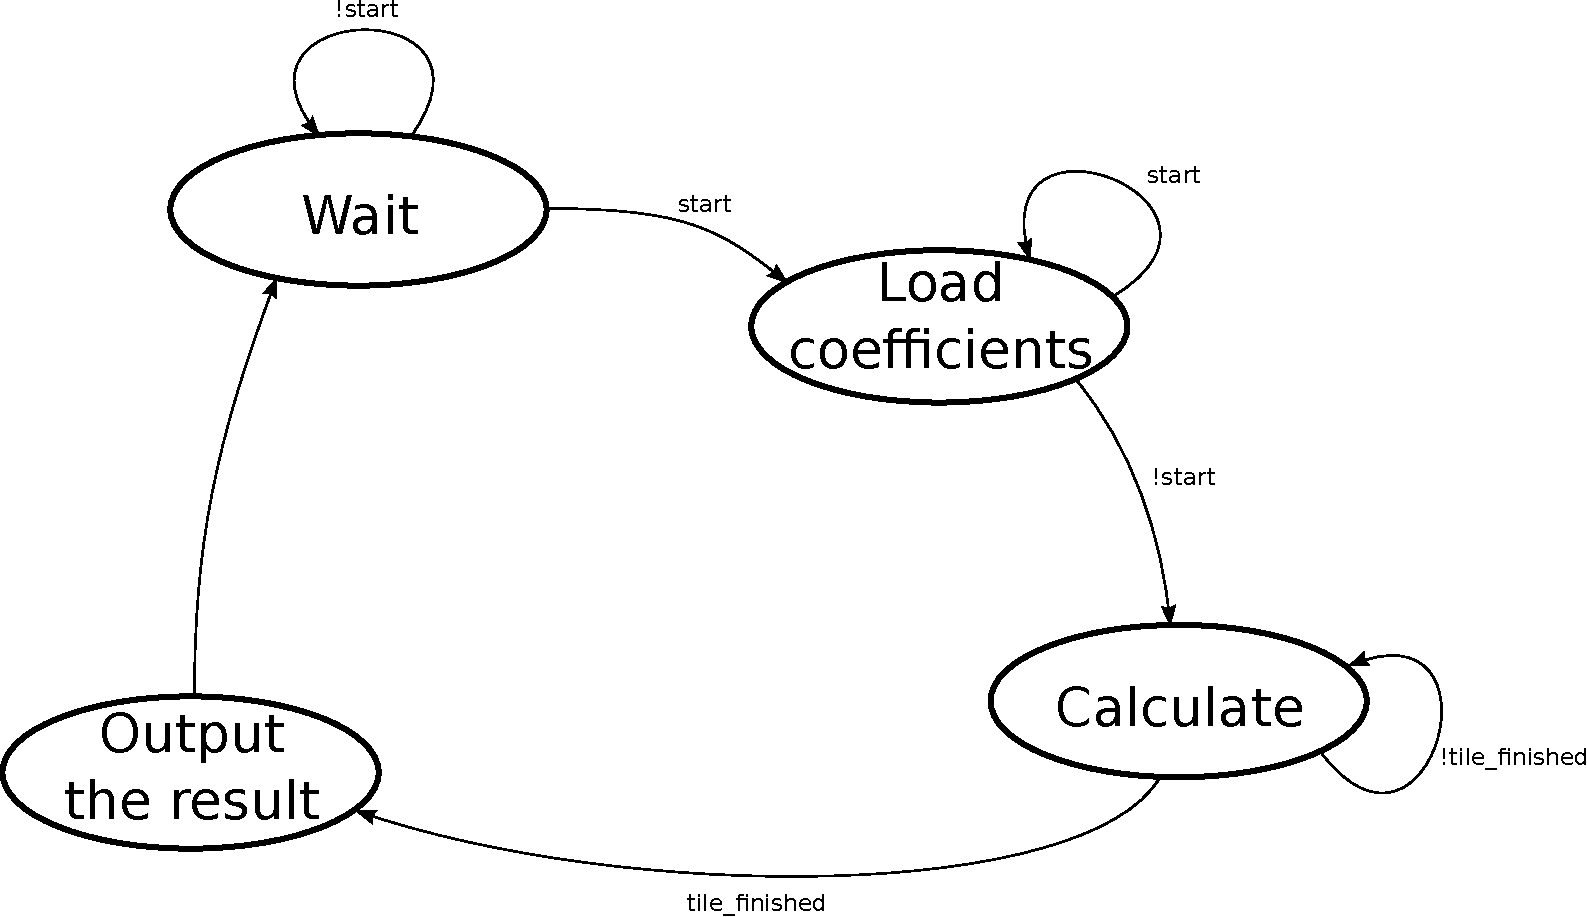
\includegraphics[width=11cm]{figs/coproc_incr_sm.pdf}
\caption{Coprocessor incremental calculation state machine}
\label{incr_sm}
\end{figure}

The module outputs both the x- and y-coordinates by the means of two processes running in parallel (\texttt{$calc_x$} and \texttt{$calc_y$}). In the slave module, the y-coordinates are stored with an address offset of 40, and two separate sets of internal registers are allocated. Therefore, no conflicts can occur.

To test the operation of the incremental calculation module, we have written a dedicated test-bench in SystemC which uses a formula to calculate the output x-coordinate directly for a given x and y output coordinates and coefficients. We initialised the Coprocessor thanks to a function which calculated the coefficients to be used by the incremental calculation module. This already allowed us to verify the functionality of the formulas using the mfixed type, which is going to be used by the LM32 for its coefficient calculations as well. It was sufficient to test the x-coordinate only since both the x and y coordinate follow the same principle. In particular, we used it to verify that the error between expected and observed value was not greater than 3\%; a value we judged acceptable. Errors are introduced due to the incremental calculation formula itself as well as the truncation in the mfixed format.

\subsubsection{Module's configuration: multiple register slave}



The configuration is transmitted to the module using a wishbone slave including multiple registers.
The coefficient slave has 20 internal registers to buffer the values calculated by the LM32 (10 for the x and 10 for the y coordinates) until they are accessed by the incremental calculation module. The module uses two internal registers: If 20 coefficients have been written, the ready signal is set high. This indicates the coprocessor that it can load these and start its calculations. In any case, all 20 coefficients must be set in a burst, i.e. writing to one register will set the ready signal down automatically until all 20 coefficients have been written. Nevertheless, no effort has been made to verify that 20 different registers have been written to and the responsibility lies with the LM32. Similarly, the internal loaded register indicates if 20 reads have been performed. The objective is to inform the LM32 if the coefficients have been loaded by the coprocessor and can thus be overwritten by new ones.

\subsection{Interpolator}

\begin{figure}[H]
\center
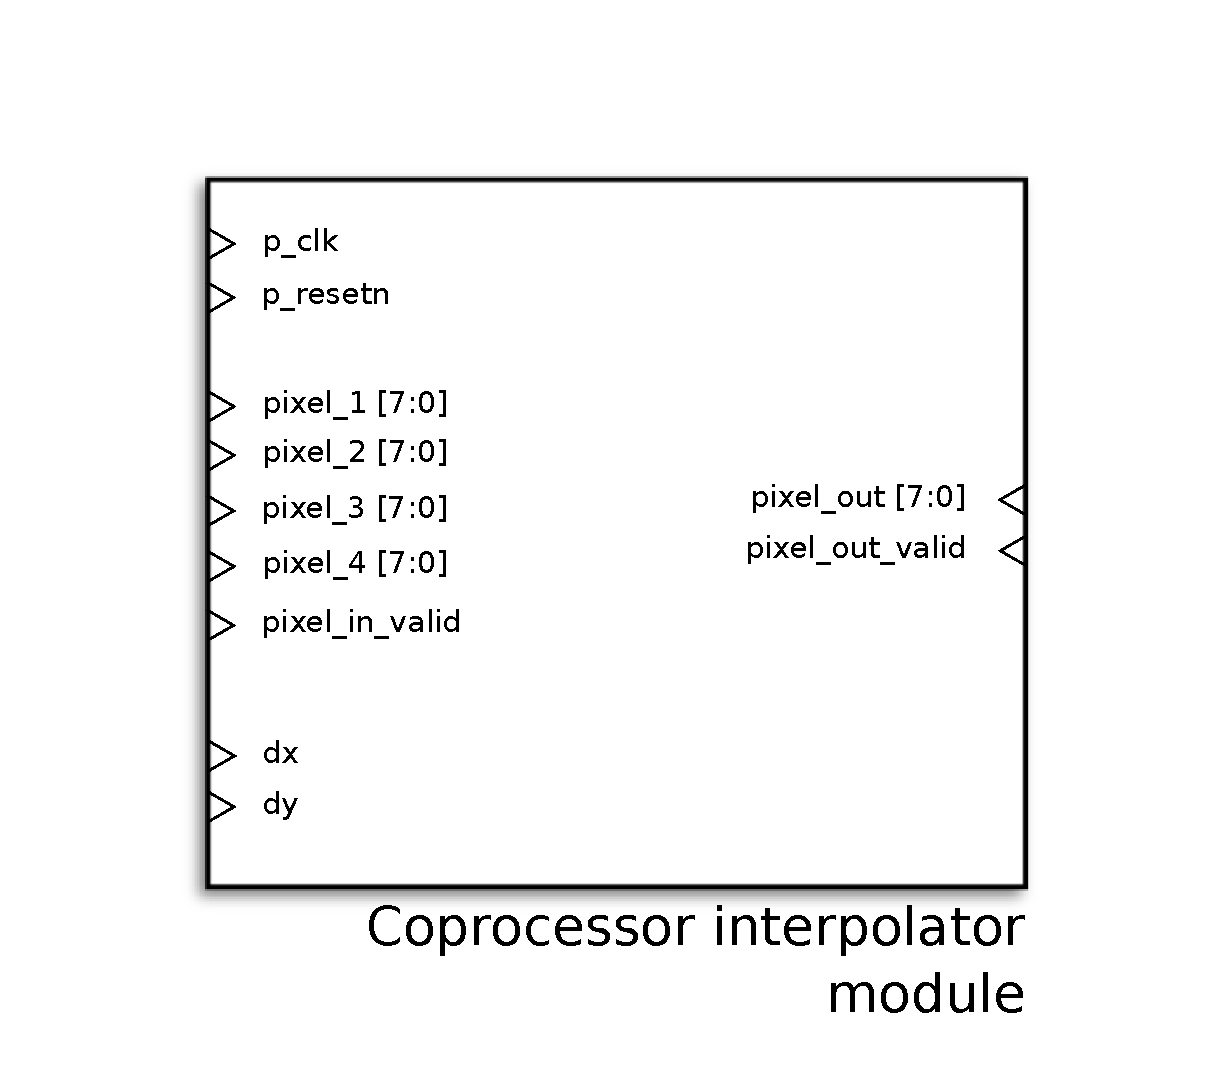
\includegraphics[width=7cm]{figs/INTERPOLATOR.pdf}
\caption{Coprocessor interpolator's interface}
\label{interpo_ports}
\end{figure}



This module consists of a single thread (\texttt{interpolate}) which is responsible for the bilinear interpolation of the fictional pixel. 

On the rising edge of the system clock, and when the input pixels(\texttt{pixel\_0, pixel\_1, pixel\_2, pixel\_3, dx, dy}) are declared as valid (\texttt{pixel\_in\_valid}), the interpolated value is outputted (\texttt{pixel\_out}) along with a signal that defines it's value as valid (\texttt{pixel\_out\_valid}). 
This operation is performed at the rate of 100MHz.  


An alternative implementation that was considered and tested was that of a module that accumulates partial results of the interpolation and creates an outputs pixel at the rate of 25MHz. This architecture is quite convenient since it only requires one inputed pixel at each rising edge of the clock. This fact could lead to a less costly and more compact design of the coprocessor.  

\subsection{Interpolator output module}

\begin{figure}[H]
\center
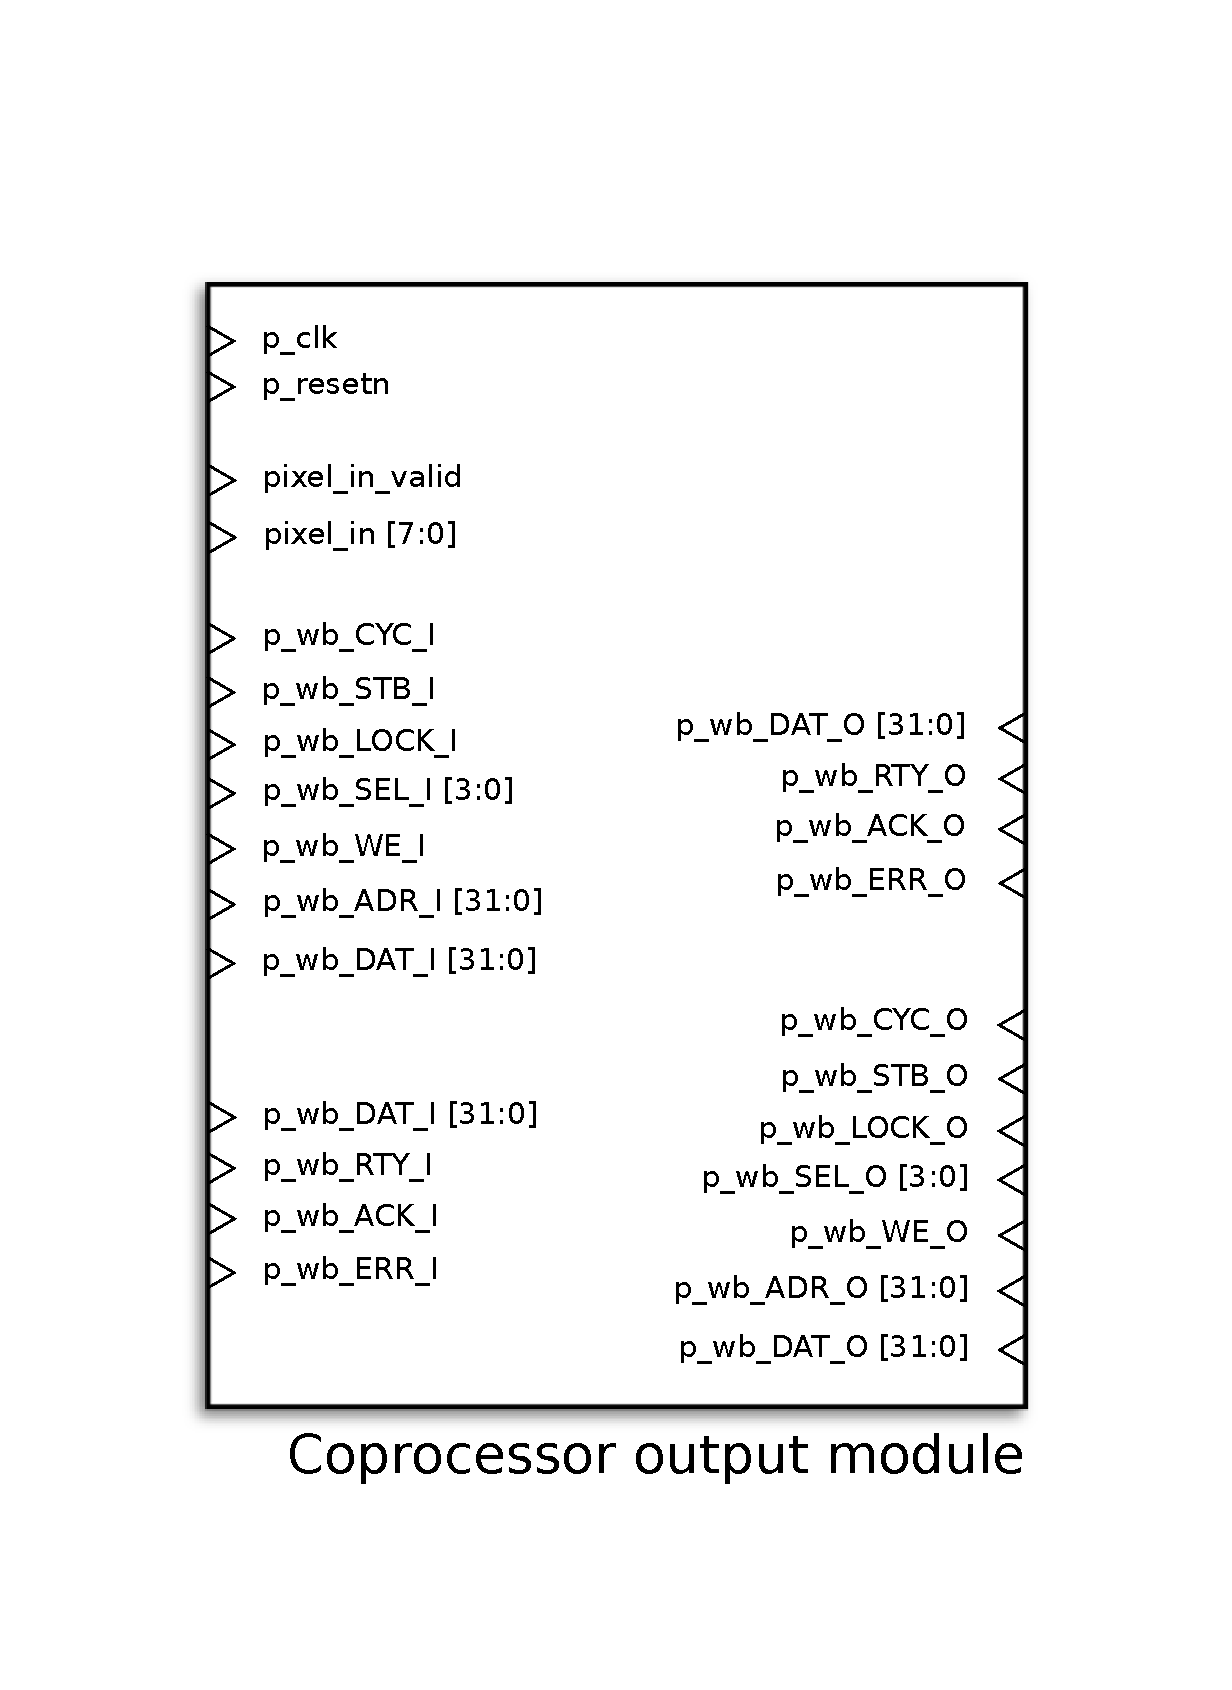
\includegraphics[width=7cm]{figs/INTERPOLATOR_OUT.pdf}
\caption{Coprocessor interpolator out module's interface}
\label{interpo_out_ports}
\end{figure}



The interpolator out module consists of two threads. 

The \texttt{process\_write\_buffer()} thread is responsible of acquiring pixels inputed by the interpolator and storing them in to the local buffer. Pixels inputed to the module (\texttt{pixel\_in}) are stored if the corresponding valid signal is true (\texttt{pixel\_valid}). The \texttt{process\_load\_buffer\_to\_ram()} thread is responsible of storing the locally stored pixels into the RAM. This is done in a tile by tile fashion. The ram memory address in which the image should be saved is stored in a register attached to the wishbone bus and therefore controlled by the processor. 

The \texttt{process\_load\_buffer\_to\_ram} module consults the content of this register once it has finished sending a complete image.

\subsection{Buffer management}

\begin{figure}[H]
\center
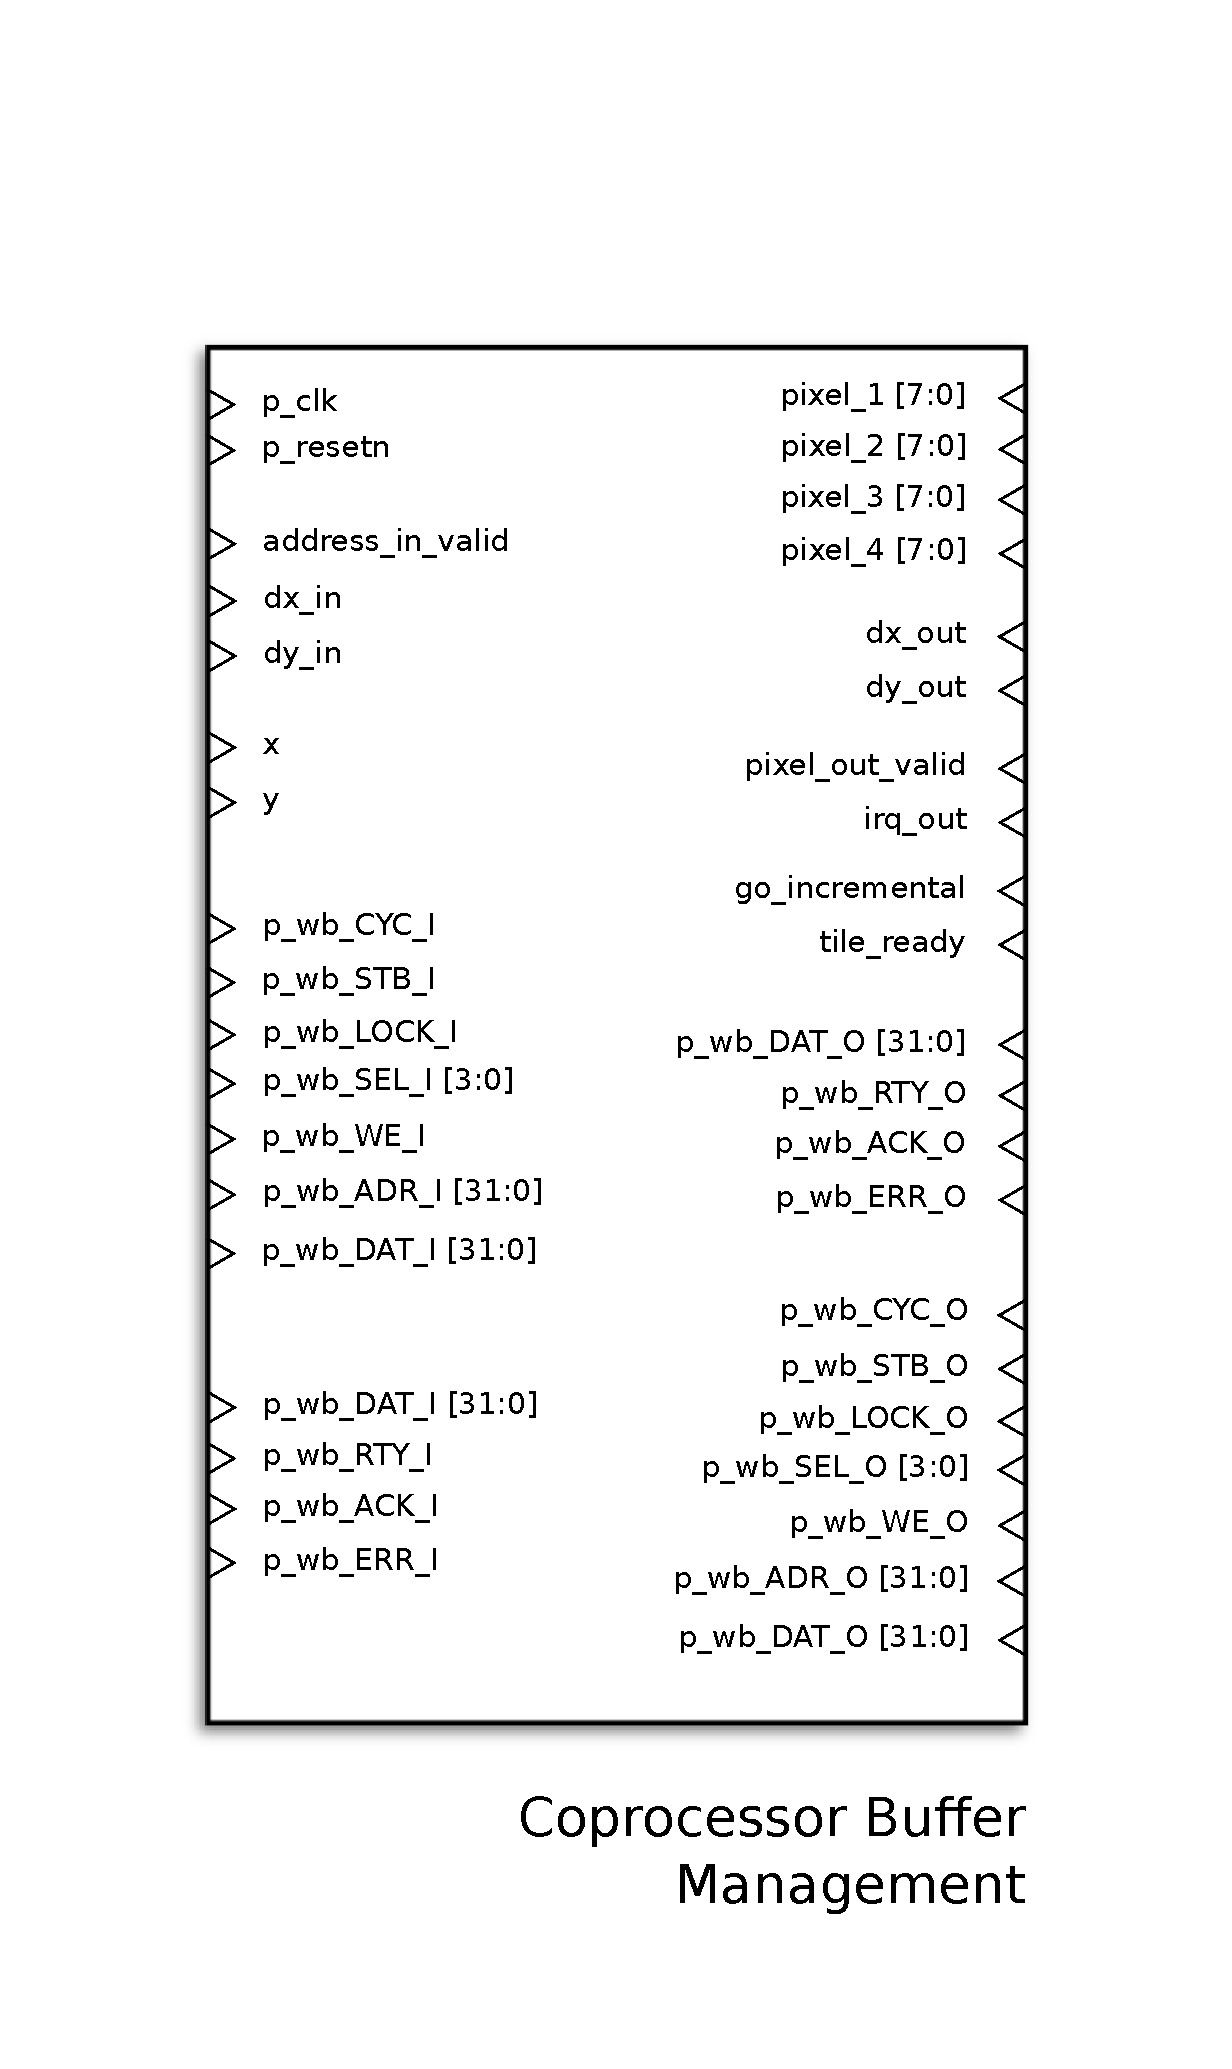
\includegraphics[width=6.9cm]{figs/Buffer_management.pdf}
\caption{Coprocessor buffer management module's interface}
\label{buff_out_ports}
\end{figure}


The \texttt{buffer\_management} module is responsible of loading the local co-processor buffer in a tile by tile fashion and performing the pixel-address to pixel value transformation. The size of the buffer is equal to 2 tiles. At each instant, one part of the buffer is used as a look-up table for the interpolator module while the other part is used as storage place for the pre-fetching of the next tile. 

The process \texttt{load\_buffer\_from\_ram} pre-fetches tiles  to be "looked-up". The address of the tile to be pre-fetched is stored in a register attached to the wishbone bus, therefore the processor (LM32) controls the contents of this register. Once the next tile to be "looked-up" has been fetched, this thread consults the content of the register and waits till the current lookup procedure has finished. 

The  \texttt{process\_lookup\_pixel\_intensity}  processor performs the lookup function. Once a tile has been looked up an interrupt is raised notifying therefore the processor. The processor should respond to this interrupt by providing the address of the next tile to be pre-fetched. 

The \texttt{process\_lookup\_pixel\_intensity} process is not allowed to lookup the next tile, unless that tile has been loaded. In this case the incremental calculation module is halted by setting the \texttt{go\_incremental} signal to false.  
